\documentclass[]{article}

\usepackage[margin=1.0in]{geometry}
\usepackage{amsmath}
\usepackage{amsfonts}
\usepackage{amsthm}
\usepackage{graphicx}
\usepackage{amssymb}

\usepackage{mathtools}

%opening
\title{Circle Packing Notes}
\author{Alex Karlovitz}
\date{}

\begin{document}
	
	\maketitle
	
\section*{Overview}

(Kontorovich's Letter to Baragar): Given a circle packing in the form of a Coxeter diagram, can produce a realization of the packing in the plane. This can be recognized as the orbit of circles in a ``cluster'' under reflections by circles in the ``co-cluster.''

(Kontorovich's Letter to Bill Duke): Then we can write down inversive coordinates.

Then we single out two circles in the cluster, say with inversive coordinates $v$ and  $v_0$, and look at the stabilizer of $v$ acting on $v_0$.
We're interested in what bends appear in this specific orbit.

Key idea: if we could somehow parametrize the stabilizer group, then perhaps the set of bends could be written as the values of some function on those parameters.
In particular, by looking at the spin representation of the stabilizer group, we can often recognize it as a congruence group (which is easy to parametrize).
One can show that the set of bends will contain the values of a shifted quaternary quadratic form (if $v_0$ is tangent to $v$, it ends up being binary).

\section*{Detailed Example}

We will consider the Apollonian packing.

Coxeter diagram: INSERT IMAGE.

Cluster/co-cluster: see Figure \ref{c-coc_Ap}.

\begin{figure}[h]
	\centering
	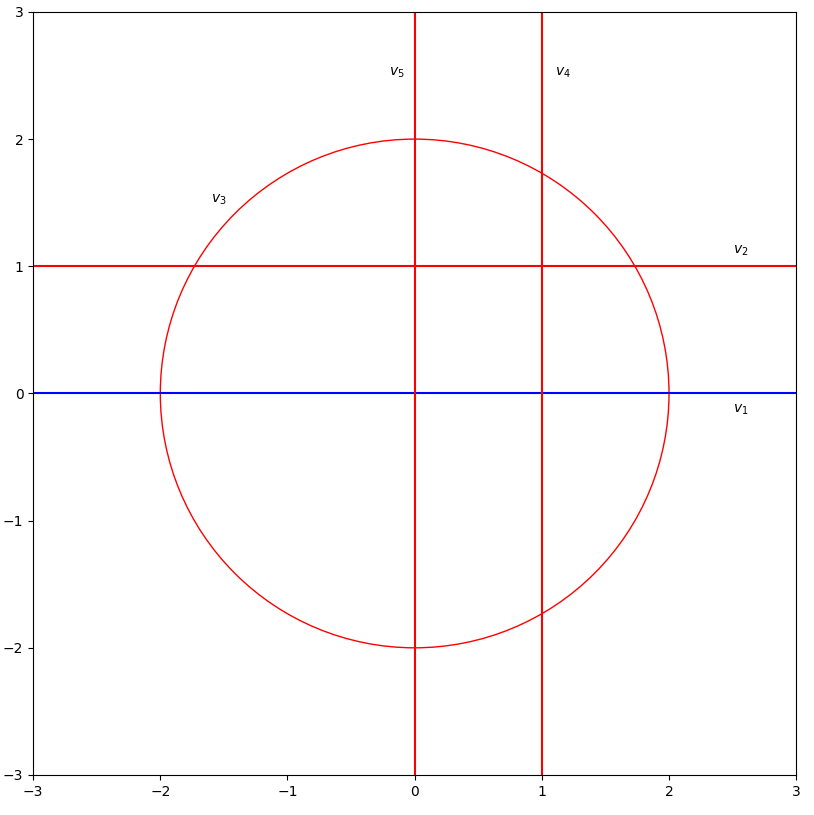
\includegraphics[width=0.6\linewidth]{c-coc_Ap.png}
	\caption{A cluster/co-cluster decomposition for the Apollonian packing.}
	\label{c-coc_Ap}
\end{figure}

Note: we write inversive coordinates as
$$
v = \left( \frac{1}{r}, \frac{x}{r}, \frac{y}{r}, \frac{1}{\hat{r}} \right)
$$
where $r$ is the radius, $(x, y)$ are the coordinates of the center, and $\hat{r}$ is the co-radius (radius of the circle after inversion through the unit circle).
These lie on the set $Q(v) = -1$ where $Q$ is the quadratic form with half-Hessian
$$
\begin{pmatrix}
~ & ~ & ~ & \frac{1}{2} \\
~ & -1 & ~ & ~ \\
~ & ~ & -1 & ~ \\
\frac{1}{2} & ~ & ~ & ~
\end{pmatrix}
$$
This realization has inversive coordinates
\begin{align*}
v_1 &= (0, 0, -1, 0) \\
v_2 &= (0, 0, 1, 2) \\
v_3 &= (1/2, 0, 0, -2) \\
v_4 &= (0, 1, 0, 2) \\
v_5 &= (0, -1, 0, 0)
\end{align*}
where $\mathcal{C} = \{v_1\}$ is the cluster and $\hat{\mathcal{C}} = \{v_2, v_3, v_4, v_5\}$ is the co-cluster.

The reflection of a circle with inversive coordinates $x$ through the circle with inversive coordinates $v$ is given by (see Letter to Baragar) $x \mapsto xR_v$ where
$$
R_v = I + 2Qv^tv
$$
Note: all such reflections have determinant $-1$.
One way to see this is to compute the eigenvalues.
Mathematica gives the eigenvalues $\{1, 1, 1, Q(v)\}$.
So if $v$ is a vector giving inversive coordinates, then $Q(v) = -1$ and $\det R_v = -1$.

The circle packing is generated by acting on the cluster by the group
$$
\Gamma = \langle R_2, R_3, R_4, R_5 \rangle
$$
That is, $\Gamma$ is generated by reflections through circles in the cocluster.

Also, note that $R_v \in O(Q)$ for any inversive coordinates $v$.
This is seen by using the fact that $vQv^t = -1$ and checking that
$$
R_vQR_v^t = Q
$$
Therefore even words in the $R_v$ live in $SO(Q)$.

Let's take two tangent circles in the packing, say $v = v_1$ and $v_0 = v_1R_{v_2}$.
Now we'll act on $v_0$ by the stabilizer of $v$. By looking at the image of the cluster/co-cluster in the plane, one sees that the stabilizer of $v_1$ is
$$
\text{Stab}(v_1) = \langle R_3, R_4, R_5 \rangle
$$
We are interested in parametrizing the stabilizer to get a nice formula for what bends appear in this orbit.
To do this, we look at
$$
\Gamma_0 = \langle R_5R_3, R_5R_4 \rangle
$$
since this is a subgroup of $\text{SO}(Q)$, meaning we can look at its pre-image under the spin representation.

\subsection*{The Spin Representation}

Observe that the matrix
$$
M =
\begin{pmatrix}
x & y + iz \\
y - iz & w
\end{pmatrix}
$$
has determinant $Q(x, y, z, w)$.
We can define a right action on such $M$ by $\text{SL}_2(\mathbb{C})$ via
$$
M.g = g^*Mg
$$
Note that the image $M.g$ is still Hermitian, and hence can be written in the form
$$
\begin{pmatrix}
x' & y' + iz' \\
y' - iz' & w'
\end{pmatrix}
$$
So each $g \in \text{SL}(2, \mathbb{C})$ defines a linear transformation
$$
\begin{pmatrix}
x & y & z & w
\end{pmatrix} \mapsto
\begin{pmatrix}
x' & y' & z' & w'
\end{pmatrix}
$$
In other words, we have defined a 4-dimensional representation $\rho$ of $\text{SL}(2, \mathbb{C})$, the so-called \textit{spin representation}.
One can of course write down this representation explicitly.
If
$$
g = 
\begin{pmatrix}
a + \alpha & b + \beta \\
c + \gamma & d + \delta
\end{pmatrix}
$$
then
$$
\rho(g) =
\begin{pmatrix}
a^2 + \alpha^2 & ab + \alpha\beta & a\beta - b\alpha & b^2 + \beta^2 \\
2(ac + \alpha\gamma) & ad + bc + \alpha\delta + \beta\gamma & a\delta - b\gamma + c\beta - d\alpha & 2(bd + \beta\delta) \\
2(-a\gamma + c\alpha) & -a\delta - b\gamma + c\beta + d\alpha & ad - bc + \alpha\delta - \beta\gamma & 2(-b\delta + d\beta) \\
c^2 + \gamma^2 & cd + \gamma\delta & c\delta - d\gamma & d^2 + \delta^2
\end{pmatrix}
$$
One easily checks that
$$
\rho
\begin{pmatrix}
0 & -2 \\
\frac{1}{2} & 0
\end{pmatrix} = R_5R_3 ~~~~~~~~
\rho
\begin{pmatrix}
1 & 2 \\
0 & 1
\end{pmatrix} = R_5R_4
$$
where $R_3, R_4, R_5$ are as before.
\\

Next, we notice that $\Gamma_0$ (the group generated by $\rho^{-1}(R_5R_3)$ and $\rho^{-1}(R_5R_4)$) is isomorphic to $\text{SL}(2, \mathbb{Z})$.
This is seen by conjugating by the matrix
$$
B =
\begin{pmatrix}
\frac{1}{\sqrt{2}} & 0 \\
0 & \sqrt{2}
\end{pmatrix}
$$
Specifically,
$$
\text{SL}(2, \mathbb{Z}) =
B^{-1}\rho^{-1}(\Gamma_0)B
$$

\subsection*{Examples of Quadratic Forms}

Next, we can parametrize SL$(2, \mathbb{Z})$ to get a quadratic form of bends.
This proceeds as follows.
Let
$$
g =
\begin{pmatrix}
a & b \\
c & d
\end{pmatrix}
$$
be an arbitrary matrix in SL$(2, \mathbb{Z})$.
Then
$$
\gamma_g := \rho\left( BgB^{-1} \right) \in \Gamma_0
$$
Thus, we can take any vector $v$ of inversive coordinates for a circle in the packing and act on it by $\gamma_g$ to produce another vector for a circle in the packing.
By leaving $g$ arbitrary, this will describe the entire orbit $v\Gamma_0$ in terms of $a, b, c$, and $d$.
By taking the first component of these vectors of inversive coordinates, we get a quadratic form of bends which appear in the packing.
\\

We can get a larger variety of bends by looking at subgroups other than $\Gamma_0$.
One simple way to get another subgroup is to conjugate $\Gamma_0$ by any matrix $W \in \Gamma$.
Notice that
$$
W^{-1}\Gamma_0W = \text{Stab}(v_1W)
$$
So by switching to this other subgroup, we are looking at the collection of bends in the orbit of $v$ under the stabilizer of $v_1W$.
\\

Let's look at some examples.
In the following figures, we plot $v$ in red and $v_1W$ in yellow.
In Figure \ref{simple}, we consider the case where $v$ and $v_1W$ are the horizontal lines.
This results in a quadratic form in just one variable.

In Figure \ref{tangent}, we look at the case where $v$ and $v_1W$ are tangent.
Here, we get a quadratic form which is binary after a simple change of variables.

In Figure \ref{non_tangent}, we consider an example where $v$ and $v_1W$ are not tangent.
This results in a nondegenerate quaternary form.

\begin{figure}[h]
	\centering
	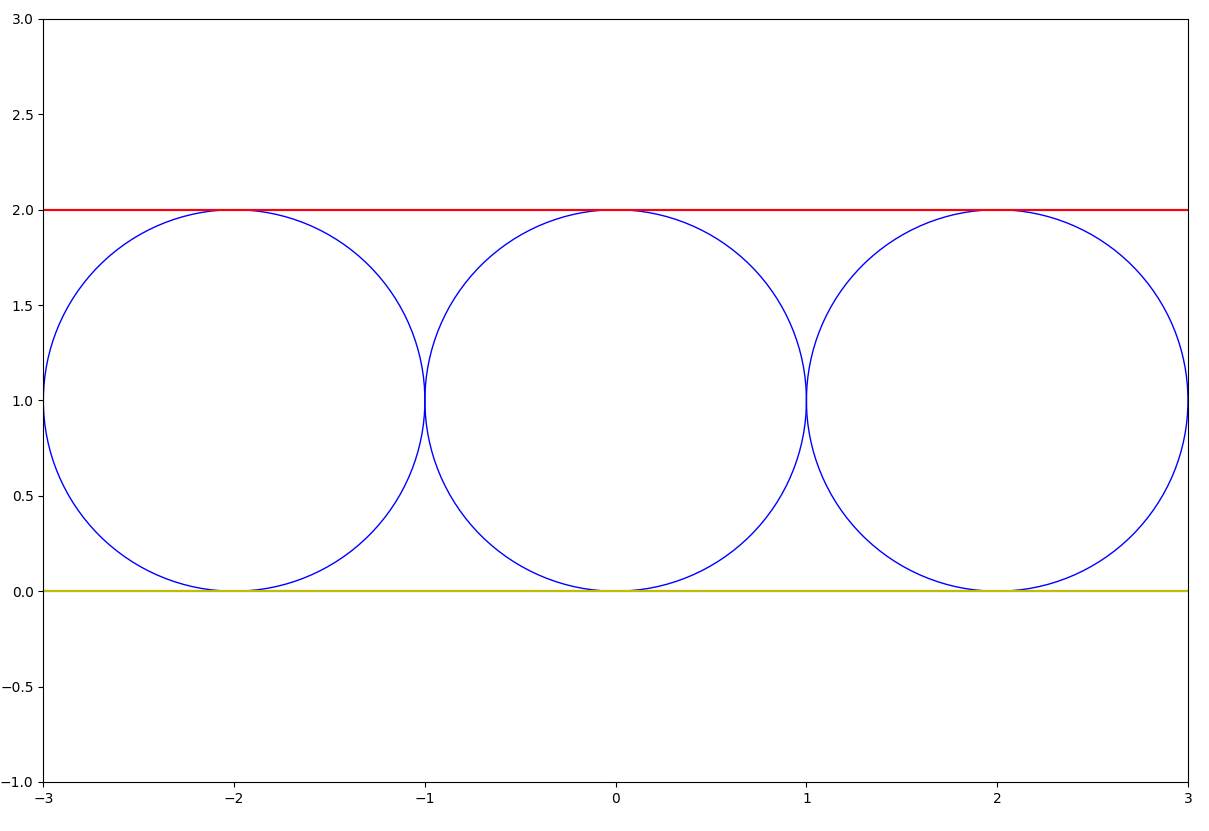
\includegraphics[width=0.8\linewidth]{simple_Ap.png}
	\caption{$ ~~~~~ v = v_1R_2 ~~~~~ W = I ~~~~~ b = c^2$}
	\label{simple}
\end{figure}
\begin{figure}[h]
	\centering
	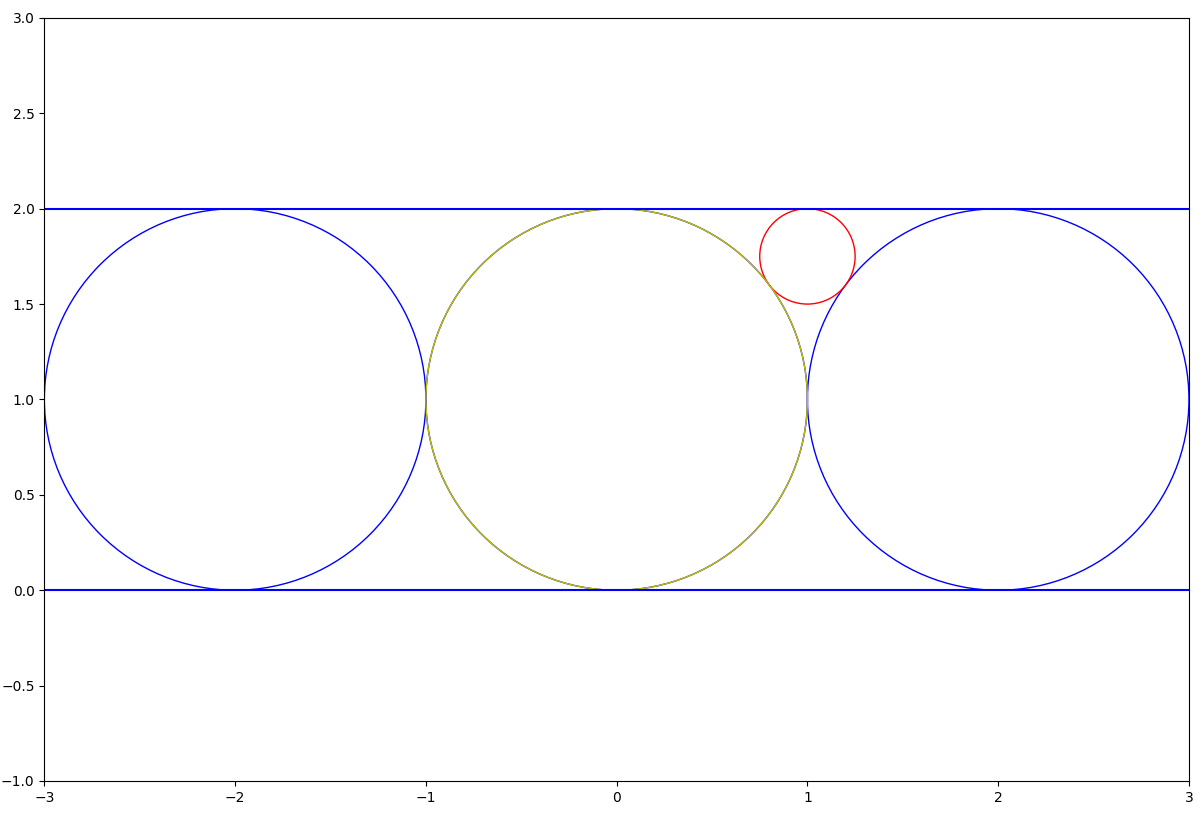
\includegraphics[width=0.8\linewidth]{tangent_Ap.png}
	\caption{$ ~~~~~ v = v_1R_2R_3R_4R_5R_4R_3R_2 ~~~~~ W = R_2R_3 ~~~~~ b = (2a + c)^2 + (2b + d)^2 - 1$}
	\label{tangent}
\end{figure}
\begin{figure}[h]
	\centering
	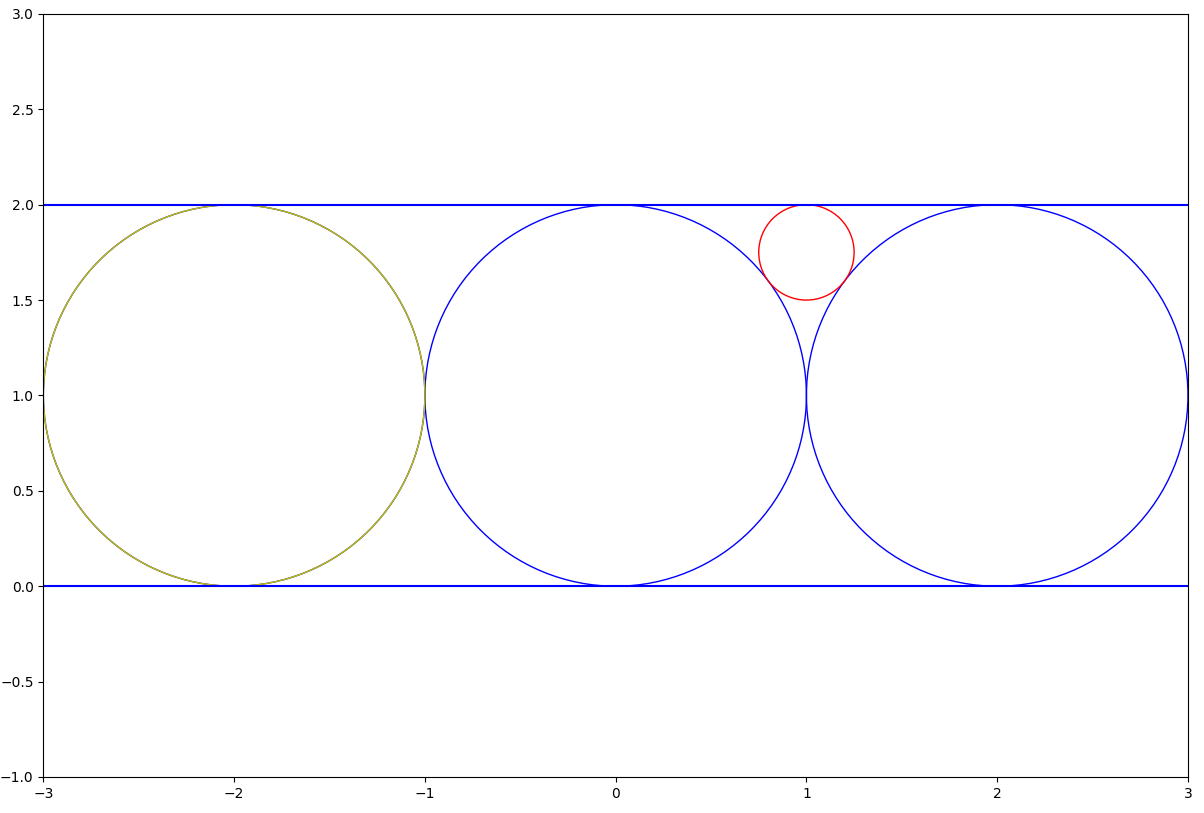
\includegraphics[width=0.8\linewidth]{non_tangent_Ap.png}
	\caption{$ ~~~~~ v = v_1R_2R_3R_4R_5R_4R_3R_2 ~~~~~ W = R_2R_3R_4R_5 ~~~~~ b = -17 + 12a^2 + 12b^2 + 12ac + 9c^2 + 12bd + 9d^2$}
	\label{non_tangent}
\end{figure}

The three examples seem to suggest two causes of degeneracy:
\begin{enumerate}
	\item Either $v$ or $v_1W$ having zero curvature
	\item $v$ and $v_1W$ being tangent
\end{enumerate}
We are interested in verifying these conditions.
	
\end{document}